\documentclass[a4paper,french,towsides,10pt]{book}
\usepackage[utf8]{inputenc}
\usepackage[french]{babel}
\usepackage{fancyhdr}
\usepackage{graphicx}
\usepackage{multirow}
\usepackage{placeins}
\usepackage[bookmarks=true]{hyperref}
\hypersetup{pdfborder={0 0 0}}
\pagestyle{fancy}
\setlength{\parskip}{1.5ex plus .4ex minus .4ex}
\renewcommand{\labelitemi}{\textbullet}
\renewcommand{\chaptermark}[1]{\markboth{#1}{}}



\pagestyle{fancy}

\renewcommand{\chaptermark}[1]{\markboth{#1}{}}
\renewcommand{\sectionmark}[1]{\markright{\thesection\ #1}}

\fancyhf{}

\fancyhead[RO,LE]{\thepage}
\fancyhead[LO]{\leftmark}
\fancyhead[RE]{Titre du livre}

\fancypagestyle{corps}{ 
\fancyhead[RO,LE]{\thepage}
\fancyhead[LO]{\rightmark}
\fancyhead[RE]{\leftmark}
}

\renewcommand{\footrulewidth}{0pt} % pas de filet en bas
\fancypagestyle{plain}{ % pages de tetes de chapitre
\fancyhead{}
% supprime l’entete
\renewcommand{\headrulewidth}{0pt} % et le filet
}
\newcommand{\clearemptydoublepage}{%
	\newpage{\pagestyle{empty}\cleardoublepage}}


%Modification des marges
%\\oddsidemargin}{-2,5cm}
%\addtolength{\textwidth}{5cm}
%\addtolength{\topmargin}{-2,5cm}
%\addtolength{\textheight}{4cm}

%definition des fonctions de la page de garde
\def\blurb{%
  \begin{tabular}{l p{0.6cm} c p{0.8cm} r}
   \multirow{3}{*}{\vspace{-1.5cm}\hspace{-1cm}
\includegraphics[width=3cm]{./files/um2}} & & & &  \multirow{3}{*}{\vspace{-1.5cm}
\includegraphics[width=2cm]{./files/ufr}} \\
    & & Ministère de l'Education Nationale & & \\
    & & Université de Montpellier II & & \\ 
    & & Place Eugène Bataillon & & \\ 
    & & 34095 Montpellier Cedex 5 & & \\ 
    \vspace{0.5cm}
   \end{tabular}
  }
\def\clap#1{\hbox to 0pt{\hss #1\hss}}%
\def\ligne#1{%
  \hbox to \hsize{%
    \vbox{\centering #1}}}%
\def\haut#1#2#3{%
  \hbox to \hsize{%
    \rlap{\vtop{\raggedright #1}}%
    \hss
    \clap{\vtop{\centering #2}}%
    \hss
    \llap{\vtop{\raggedleft #3}}}}%
\def\bas#1#2#3{%
  \hbox to \hsize{%
    \rlap{\vbox{\raggedright #1}}%
    \hss
    \clap{\vbox{\centering #2}}%
    \hss
    \llap{\vbox{\raggedleft #3}}}}%

%definition du titre et autres param
\def\titre{\LARGE TP FMIN105 \\ Algorithmique / Complexité / Calculabilité}
\def\sstitre{Rapport (Décembre 2011)}
\def\auteurs{
      Thibaut \textsc{Marmin} \\
      Clément \textsc{Sipieter} \\
      Williman \textsc{l'Australien}}

\begin{document}
\renewcommand{\labelitemii}{\textasteriskcentered}
\thispagestyle{empty}
  \vbox to .9\vsize{%
  \vss
  \vbox to 1\vsize{%
    \haut{}{\blurb}{}
    \vfill
    
    \noindent\rule{\linewidth}{.5pt}
    \ligne{\vspace{1.5mm}\titre}
    \noindent\rule{\linewidth}{.5pt}
    \ligne{\normalsize{\textsc{\sstitre}}}
    \vfill
    \ligne{%
      \begin{tabular}{l}
	\vspace{5mm}
      \end{tabular}
      \begin{tabular}{c}
      Travail préparé par : \\\\
       \auteurs
      \end{tabular}
    }
  \vss
  }
}
\clearemptydoublepage
\tableofcontents
\clearemptydoublepage
\chapter{Partie théorique}

\section{Partie algorithmique}
\begin{enumerate}
\item Le nombre de manières de colorier un graphe est le produit des nombres de façons de colorier chaque arc.
\begin{itemize}
\item Si le graphe $G$ est complet, on aura $k$ couleurs possibles pour le premier sommet, $(k-1)$ pour le deuxième, etc\ldots (Le graphe G étant complet, la couleur du premier sommet est nécessairement exclu des autres sommets)

Le $n$\^{ième} sommet pourra être colorié de $k-(n-1)$ manières. D'où :
\[ P_{K_n}(k)=\prod_{i=0}^{n-1}(k-i) \]

\item Si $G$ est vide, la coloration d'un sommet ne contraint pas la coloration des autres sommets. On obtient alors :
\[ P_{\overline{K_n}}(k)=k^n \]
\end{itemize}
\item $\chi(G)$ étant, par définition, le nombre minimum de couleurs nécessaires pour colorier $G$, si $k < \chi(G)$ alors le graphe $G$ ne peut pas être colorié par $k$ couleurs. Si $k \geq \chi(G)$ alors il doit y avoir au moins une manière de colorier $G$, celui utilisant $\chi(G)$ couleurs.

On a donc :
\begin{displaymath}
	P_G(k) \left\{ \begin{array}{ll}
	=0 & \textrm{si $k < \chi(G)$} \\
	\geq 1 & \textrm{sinon}
	\end{array} \right.
\end{displaymath}

\item Montrons d'aboard que la propriété est vraie pour tout graphe complet $K_n$. Pour commencer on remarque que, pour tout arrête $e$:

\begin{itemize}
\item $K_{n\backslash e}$ est exactement $K_{n-1}$, et donc: 

\[ P_{K_n\backslash e}(k) = P_{K_{n-1}} = \prod_{i=0}^{n-2}(k-i) \]


\item Soit $e = (a,b)$. On peut supposer (sans perte de généralité) que $b$ est considéré en dernier lors de la coloration de $K_n$, donc qu'il lui reste $k-(n-1)$ couleurs. Pour colorier $K_{n-e}$ on aura un choix de plus pour lui, à savoir la couleur de $a$, donc $k-(n-2)$ en totale. De ce fait:

\[ P_{K_n-e}(k) = P_{K_{n-1}}(k)(k-(n-2)) = (\prod_{i=0}^{n-2}(k-i))(k-(n-2)) \]
\end{itemize}

On a donc très clairement:
\begin{eqnarray*}
P_{K_n-e}(k) -  P_{K_n\backslash e}(k) &=& (\prod_{i=0}^{n-2}(k-i))(k-(n-2)) - \prod_{i=0}^{n-2}(k-i)\\
&=& \prod_{i=0}^{n-2}(k-i)(k-(n-1))\\
&=& \prod_{i=0}^{n-1}(k-i)\\
&=& P_{K_n}(k)
\end{eqnarray*}
Tout graphe de rang $n$ pouvant se générer à partir de $K_n$ (en enlevant des arrêtes) on cherchera à prouver que la suppression d'arrête conserve notre propriété. Autrement dit on aimerait montrer que pour tout graphe $G$ et tout arrête $a$ de celui-ci:

\begin{eqnarray*}
&&P_G(k) = P_{G-e}(k) - P_{G \backslash e}(k) \\
&\Rightarrow&  P_{G-a}(k) = P_{G-e-a}(k) - P_{G \backslash e-a}(k)
\end{eqnarray*}

On supposera évidemment que $a$ et $e$ sont distinctes. 

TODO FINISH

\item Soit $H$ un prédicat tel que :
\begin{displaymath}
	H(m) \left\{ \begin{array}{ll}
	\top & \textrm{si $\forall$ $G$, graphe de $m$ arrêtes ou moins, $P_G(k)$ est polynomiale.} \\
	\bot & \textrm{sinon.}
	\end{array} \right.
\end{displaymath} 
\begin{itemize} 
\item Nous rappellons que $P_{\overline{K_n}}(k)=k^n$, donc $H(0)$ est vraie. 
\item Supposons $\exists m \in \mathbb{N}$ $|$ $H(m)$ l'est également. Soit $G_{m+1}$ un graphe à $m+1$ arrêtes:

\[ P_{G_{m+1}} = P_{G_{m+1}-e} - P_{G_{m+1} \backslash e} \]

Clairement $P_{G_{m+1}-e}$ et $P_{G_{m+1} \backslash e}$ ont $(m+1)-1 = m$ arrêtes. Or par hypothèse de recurrence $H(m)$ est vraie,
$P_{G_{m+1}}$ est la différence entre deux polynomiales, donc est polynomiale lui-même. On a donc $H(m+1)$.
\item On vient de montrer $H(0) \wedge (H(m) \Rightarrow H(m+1))$. Par récurrence on a donc $H(m) \forall m \in \mathbb{N}$. 

\end{itemize} 



\item Utilisons la formule trouvée au point précédent, et admettons que pour $P_n$ une chaîne de taille $n$ on a :
\[ P_n(k) = k(k-1)^{n-1} \]

Prenons $A$ le graphe initial :
\begin{eqnarray*}
P_A(k) & = & P_B(k) - P_C(k) \\
&=& \big(P_D(k)-P_E(k)\big)-\big(P_F(k)-P_{P_3}(k)\big)\\
&=& \Big[\big(P_{P_5}(k)-P_{P_4}(k)\big)-\big(P_{P_4}(k)-P_{P_3}(k)\big)\Big]-\Big[\big(P_{P_4}(k)-P_{K_3}(k)\big)-P_{P_3}(k)\Big]\\
&=& P_{P_5}(k)+2P_{P_3}(k)-P_{K_3}(k)+3P_{P_4}(k)\\
&=& k(k-1)^4 +2k(k-1)^2+k(k-1)(k-2)-3(k-1)^3 \\
&=& k(k-1)\big[(k-1)^3+z(k-1)+(k-z)-3(k-1)^2\big]\\
&=& (k^2-k)\Big[(k-1)^2\big((k-1)-3\big)+3k -4 \Big]\\
&=& (k^2-k)[k^3-6k^2+12k-8]\\
&=& k^5-7k^4+18k^3-20k^3+8k
\end{eqnarray*}
Où :

$A$ : \raisebox{-0.5\height}{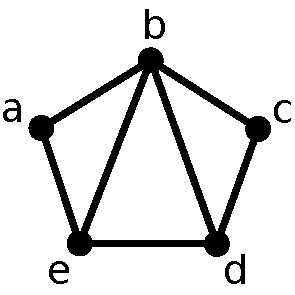
\includegraphics[width=2cm]{files/gAex1.pdf}}

\begin{tabular}{llcll}
$B = A-(e,d) $ : & \raisebox{-0.5\height}{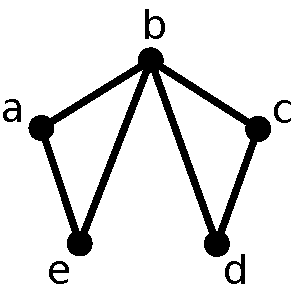
\includegraphics[width=2cm]{files/gBex1.pdf}} & et & $C = A\backslash(e,d)$ : & \raisebox{-0.5\height}{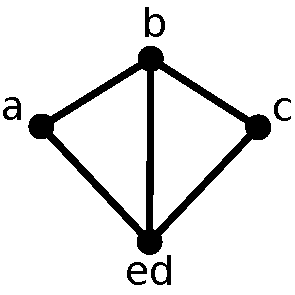
\includegraphics[width=2cm]{files/gCex1.pdf}} \\
$D = C-(a,b)$ : & \raisebox{-0.5\height}{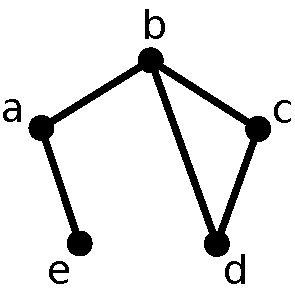
\includegraphics[width=2cm]{files/gDex1.pdf}} & et & $E = C\backslash(e,b)$ : & \raisebox{-0.5\height}{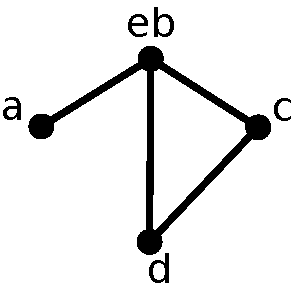
\includegraphics[width=2cm]{files/gEex1.pdf}} \\
$F = C-(b,ed)$ : & \raisebox{-0.5\height}{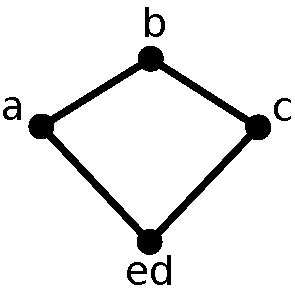
\includegraphics[width=2cm]{files/gFex1.pdf}}& et & $C \backslash(b,ed)P_3$ : & \raisebox{-0.5\height}{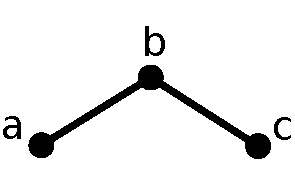
\includegraphics[width=2cm]{files/gC-ex1.pdf}}
\end{tabular}
\end{enumerate}
\section{Partie complexité}
\subsection{SAT $\propto$ 3--SAT}
\begin{enumerate}[(a)]
\item \begin{description}
\item[Énoncé de SAT] : \\
\begin{tabular}{r l l}
Données : & $ \mathcal{V} = \lbrace v_1, v_2 \ldots v_n \rbrace $ & \emph{Ensemble de $n$ variables}\\
& $ \mathcal{C} = \lbrace c_1, c_2, c_3 \ldots c_m \rbrace $ & \emph{Ensemble de $m$ clauses}\\
où & $ c_i = ( l_{i1} \vee l_{i2} \vee \cdots \vee l_{ik} ) $ & \emph{Clauses de $k$ littéraux}\\
avec & $ l_{ij} = v$ ou $ \neg v $ & \emph{avec $v \in U$} \\
\end{tabular}

Problème : existe-il au moins une affectation des variables telle que chaque clause de $\mathcal{C}$ soit vrai.

\item [Énoncé de 3--SAT] : 

3--SAT est identique au problème SAT avec $k = 3$.\\
\begin{tabular}{r l}
Données : & $ \mathcal{V} = \lbrace v_1, v_2, v_3 \ldots v_n \rbrace $\\
& $ \mathcal{C} = \lbrace c_1, c_2, c_3 \ldots c_m \rbrace $\\
où & $ c_i = ( l_{i1} \vee l_{i2} \vee l_{i3} ) $\\
avec & $ l_{ij} = v$ ou $ \neg v$\\
\end{tabular}
\end{description}
\item La réduction du problème SAT peut être définit en montrant que chaque clause $c$ de $\mathcal{C}$ peut-être transformée en un ensemble de clauses $\mathcal{C'}$ tel que pour toute affectation rendant vrai l'ensemble des clauses de $\mathcal{C}$, on peut trouver une affectation rendant vrai chaque clause de $\mathcal{C'}$. Chaque clause de $\mathcal{C'}$ devant être de taille exactement 3. La réciproque doit également être montrée.

Définissons les réductions :

\begin{description}
\item \mathversion{bold} $k = 1$ \mathversion{normal}

Soit $ci_1$ une clause de taille 1, on a $ci_1 = (l)$.
Ajoutons deux variables $v_1, v_2 \notin \mathcal{V}$ et transformons la clause $c$ en quatre clauses. On obtient l'ensemble $\mathcal{C}_1 = \lbrace c_1, c_2, c_3, c_4 \rbrace$ avec :
\[ c_1 = ( l \vee v_1 \vee v_2 )\]
\[ c_2 = ( l \vee v_1 \vee \neg v_2 )\]
\[ c_3 = ( l \vee \neg v_1 \vee v_2 )\]
\[ c_4 = ( l \vee \neg v_1 \vee \neg v_2 )\]

\item \mathversion{bold} $k = 2$ \mathversion{normal}

Soit $ci_2$ une clause de taille 2, on a $ci_2 = ( l_1 \vee l_2 )$.
Ajoutons une variable $v \notin \mathcal{V}$ et transformons la clause $c$ en deux clauses. On obtient l'ensemble $\mathcal{C}_2 = \lbrace c_1, c_2 \rbrace$ avec :
\[ c_1 = ( l_1 \vee l_2 \vee v )\]
\[ c_2 = ( l_1 \vee l_2 \vee \neg v )\]

\item \mathversion{bold} $k = 3$ \mathversion{normal}

La clause $ci_3$ ne subit pas de transformation.
\[ \mathcal{C}_3 = \lbrace ci_3 \rbrace \]

\item \mathversion{bold} $k > 3$ \mathversion{normal}

Soit la clause $ci_k = ( l_1 \vee l_2 \vee \cdots \vee l_k )$. On ajoute $(k - 3)$ nouvelles variables $(v_1, v_2 \ldots v_{k-3})$.

\[ \mathcal{C}_k = \underbrace{(l_1 \vee l_2 \vee v_1)}_{c_1} \bigwedge_{i=1}^{k-4}\left[ \underbrace{(\neg v_i \vee l_{i+2} \vee v_{i+1})}_{c_{i+1}}\right]  \wedge \underbrace{(\neg v_{k-3} \vee l_{k-1} \vee l_{k})}_{c_{k-2}} \]

Montrons que SAT est vrai si et seulement si 3--SAT est vrai :

\begin{description}
 \item \textbf{SAT $\rightarrow$ 3--SAT}
 
 	\begin{itemize}
 		\item Soit une interprétation $I_1$ qui satisfasse la clause $ci_1$ :
 		 \[ val(I_1,ci_1) = val(I_1,l) = vrai\]
 		
 		Prenons une interprétation $I_1'$ avec $val(I_1,l) = val(I_1',l)$, peu importe les affectations de $v_1$ et $v_2$, $l$ étant présent dans toutes les clauses de $\mathcal{C}_1$ :
 		\[ val(I_1',\mathcal{C}) = \top \]
 		
 		\item Soit une interprétation $I_2$ qui satisfasse la clause $ci_2$ :
 		\[ \exists i, val(I_2,l_i) = \top \]
 		Prenons une interprétation $I_2'$ avec :
 		\[ val(I_2,l_1) = val(I_2',l_1) \]
  		\[ val(I_2,l_2) = val(I_2',l_2) \]
  		Peu importe l'affectation de $v$ dans $I_2'$, on a $val(I_2',\mathcal{C}_2) = \top$.
  		
  		\item Soit une interprétation $I_k$ qui satisfasse la clause $ci_k$ :
  		\[ \exists i, val(I_k,l_i) = \top \]
  		
  		Prenons une interprétation $I_k'$ telle que :
  		\begin{eqnarray*}
  		val(I_k,l_i) & = & val(I_k',l_i)  \\
  		\forall j \in \mathbb{N}^* \mid j \leq (i-2), val(I_k', v_j) & = & \top \\
  		\forall j \in \mathbb{N}^* \mid (i-1) \leq j \leq (k-3), val(I_k', v_j) & = & \bot \\
  		\end{eqnarray*}
  		
  		On obtient :
  		\[ val(I_k',\mathcal{C}_k) = \top\]
  		
 	\end{itemize}
 	
 \item \textbf{3--SAT $\rightarrow$ SAT}
 
 	\begin{itemize}
 	\item Prenons une interprétation $I_1$ telle que $val(I_1,\mathcal{C}_1) = \top$.
 	
 	Sans perte de généralité, on suppose que : 
 	\[ val(I_1,v_1) = val(I_1,v_2) = \top \]
 	La clause $c_4$ de $\mathcal{C}_1$ ne peut être satisfaite que si $val(I_1,l) = \top$.
 	
 	On a donc :
 	\[ val(I_1,ci_1) = \top \]
 	
 	\item Prenons une interprétation $I_2$ telle que $val(I_2,\mathcal{C}_2) = \top$.
 	
 	Sans perte de généralité on suppose que :
 	\[val(I_2,v) = \top \]
 	
 	La clause $c_2$ de $\mathcal{C}_2$ ne peut être satisfaire que si $val(I_2,(l_1 \vee l_2)) = \top$.
 	
 	On a donc :
 	\[ val(I_2,ci_2) = \top \]
 	
 	\item Prenons une interprétation $I_k$ telle que $val(I_k,\mathcal{C}_k) = \top$ et montrons qu'il existe forcément un $i$ tel que $val(I_k,l_i) = \top$.
 	
 	Supposons que l'interprétation $I_k$ est modèle de $\mathcal{C}_k$ avec 
 	\[ \forall i \in \mathbb{N}^* \mid i \leq k, val(I_k,l_i) = \bot \]
	\[ \Rightarrow val(I_k,v_1) = \top  \textrm{ (dans $c_1$)} \]
	Donc :
	
	\begin{tabular}{lrl}
		& $\forall i \in \mathbb{N}^* \mid i \leq (k-4), val(I_k,v_{i+1})$ & $= \top$ \\
		$\Rightarrow$ & $val(I_k,v_{k-3})$ & $= \top$ \\
		$\Rightarrow$ & $val(I_k,c_{k-2})$ & $= \bot$ \\
		$\Rightarrow$ & $val(I_k,\mathcal{C}_k)$ & $= \bot$
	\end{tabular}
	
	Pour que l'interprétation $I_k$ satisfasse $\mathcal{C}_k$, il doit exister un $i \in \mathbb{N}^*$ tel que $i \leq k$ et que $val(I_k,l_i) = \top$.
	
	On a donc :
	\[ val(I_k,ci_k) = \top \]
 	 	
 	\end{itemize}
 
\end{description}

\end{description}

\item Le point (b) définit la réduction de SAT vers 3--SAT. Afin de montrer la NP-Complétude de 3--SAT, montrons que la réduction s’effectue en un temps polynomial.

Soit :
\begin{description}
\item $k$ la taille de la clause initiale,
\item $v_k$ le nombre de variables à ajouter pour obtenir des clauses de taille 3,
\item $w_k$ le nombre de clauses de taille 3 obtenues à partir de la clause initiale.
\end{description}
\begin{center}
\begin{tabular}{c c}
$v_3 = 0$ & $w_3 = 1$ \\
$v_4 = 1$ & $w_4 = 2$ \\
$v_5 = 2$ & $w_5 = 3$ \\
\vdots & \vdots
\end{tabular}
\end{center}

Pour tout $k > 3$ :
\[ v_k = v_{\left \lceil \frac{k}{2} \right \rceil + 1} + v_{\left \lfloor \frac{k}{2} \right \rfloor + 1} + 1 \]
\[ w_k = w_{\left \lceil \frac{k}{2} \right \rceil + 1} + w_{\left \lfloor \frac{k}{2} \right \rfloor + 1} \]

$v_k = \theta(k)$, donc borné par la taille de F. La réduction s'effectue donc en un temps polynomial.

Il est possible de réduire le problème SAT à 3--SAT en un temps polynomial, SAT étant NP-complet, 3--SAT l'est aussi.
\item Soit $\mathcal{C}$ un ensemble de clause à $n_v$ variables avec $n_1$ clauses de taille 1, $n_2$ clauses de taille 2, $n_3$ clauses de taille 3, $n_4$ clauses de taille 4 et $n_5$ clauses de taille 5. Calculons le nombre de variables et le nombre de clauses obtenues après réduction (respectivement $n_v'$ et $n_c'$).

Les points (b) et (c) permettent de déterminer pour une clause de taille $k$, le nombre de clause obtenues et le nombre de variables ajoutées après réduction. On peut donc en déduire la tableau suivant :

\begin{tabularx}{\textwidth}{| X || c | c | c | c | c |}
\hline
Taille de la clause dans $\mathcal{C}$	& 1 	& 2 	& 3 	& 4 	& 5 	\\
\hline
Nombre de clauses						& $n_1$	& $n_2$	& $n_3$	& $n_4$	& $n_5$	\\
\hline
Nombre de variables ajoutées par clause	& 2		& 1 	& 0 	& 1 	& 2 	\\
\hline
\textbf{Nombre de variables ajoutées au total} 	& $2n_1$& $n_2$	& 0		& $n_4$	& $2n_5$\\
\hline
Nombre de clauses obtenues par clause 	& 4 	& 2 	& 1 	& 2 	& 3 	\\
\hline
\textbf{Nombre de clauses obtenues au total}	& $4n_1$& $2n_2$& $n_3$	& $2n_4$& $3n_5$\\
\hline

\end{tabularx}

On a donc :
\[ n_v' = n_v + 2n_1 + n_2 + n_4 + 2n_5 \]
\[ n_c' = 4n_1 + 2n_2 + n_3 + 2n_4 + 3n_5 \]
\end{enumerate}

\subsection{3--SAT $\propto$ 2--SAT ?}
Cette réduction repose sur un principe qui consiste à décomposer une clause de taille $k$ en plusieurs clauses de tailles inférieures.

Soit une clause $c = (l_1 \vee l_2 \vee l_3)$ une clause de taille 3 et $I$ une interprétation qui satisfait $c$.

\begin{description}
\item[Cas 1 :] décomposons cette clause en deux clauses $c_1$ et $c_2$ de tailles 1 et 2 :
\begin{eqnarray*}
c_1&=&(l_1) \\
c_2&=&(l_2 \vee l_3)
\end{eqnarray*}
Pour montrer l'équivalence 3--SAT $\leftrightarrow$ 2--SAT, il faut ajouter une variable $v$ aux deux clauses créées :
\begin{eqnarray*}
c_1&=&(l_1 \vee v) \\
c_2&=&(l_2 \vee l_3 \vee \neg v)
\end{eqnarray*}

On a donc la clause $c_2$ de taille 3.

\item[Cas 2 :] décomposons cette clause en trois clauses $c_1$, $c_2$ et $c_3$ de taille 1 :
\begin{eqnarray*}
c_1 & = & (l_1) \\
c_2 & = & (l_2) \\
c_3 & = & (l_3)
\end{eqnarray*}

Pour montrer l'équivalence 3--SAT $\leftrightarrow$ 2--SAT, il faut ajouter deux variables $v_1$ et $v_2$ aux trois clauses créées :
\begin{eqnarray*}
c_1 & = & (l_1 \vee v_1 \vee \neg v_2) \\
c_2 & = & (l_2 \vee \neg v_1 \vee v_2)\\
c_3 & = & (l_3 \vee v_1 \vee v_2)
\end{eqnarray*}
On a donc également des clauses de taille 3. La réduction définie ci-avant ne permet donc pas la réduction de 3--SAT vers 2--SAT.
\end{description}




\subsection{2--SAT, un problème polynomial}
\begin{enumerate}[(a)]
\item Systèmes de deux clauses à deux littéraux :
\begin{description}
\item[Insatisfiable] : $(x \vee x) \wedge (\neg x \vee \neg x)$ \\
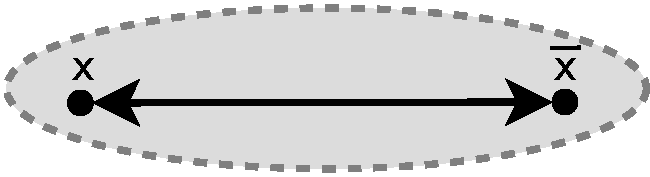
\includegraphics[width=5cm]{files/g1ex3.pdf}
\item[Valide] : $(x \vee \neg x) \wedge (\neg x \vee x)$ \\
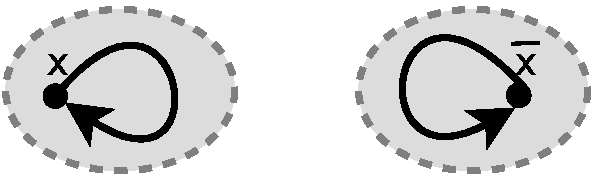
\includegraphics[width=5cm]{files/g2ex3.pdf}
\item[Contingent] : $(x \vee x) \wedge (x \vee x)$ \\
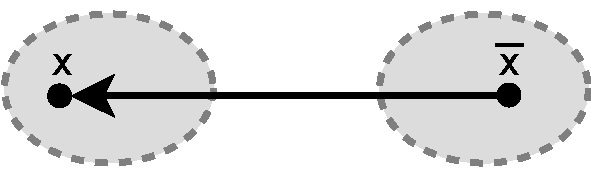
\includegraphics[width=5cm]{files/g3ex3.pdf}
\end{description}
\item 

Insaisissabilité du premier ensemble de clauses est clairement visible sur le graphe car les sommets $x$ et $\neg x$ sont dans la même composante fortement connexe.

Le deux autres ensembles sont satisfiables, les deux sommets ne sont pas dans la même composante fortement connexe.


\item L'algorithme suivant permet la génération du graphe correspondant à l'ensemble de clauses passé en paramètres, que nous appellerons graphe de satisfaction:

\begin{algorithm}[H]
  \caption{GrapheSatisfaction($\mathcal{C},\mathcal{V}$)}
  \Donnees{\\
  $\mathcal{C}$ \textit{// Ensemble de clauses}\\
  $\mathcal{V}$ \textit{// Ensemble des variables}
  }
  \Deb{
  Graphe.$\mathcal{S} = \emptyset$; \textit{// Ensemble des sommets du graphe}\\
  Graphe.$\mathcal{A} = \emptyset$; \textit{// Ensemble des arcs du graphe}\\
  \textit{// Initialisation des sommets}\\
  \PourTous{$v \in \mathcal{V}$}{
  ajouter(Graphe.$\mathcal{S}$,$v$)\;
  ajouter(Graphe.$\mathcal{S}$,$\neg v$)\;
  }
  \textit{// Parcours des clauses}\\
  \PourTous{$c \in \mathcal{C}$}{
  	ajouter(Graphe.$\mathcal{A}$,$(\neg c.x,c.y)$)\;
  	ajouter(Graphe.$\mathcal{A}$,$(\neg c.y,c.x)$)\;
  }
    \Retour Graphe\;
  }
\end{algorithm}
Cet algorithme effectue un parcours de $\mathcal{V}$ et un parcours de $\mathcal{C}$, sa complexité est donc $O(|\mathcal{C}|+|\mathcal{V}|)$.

\item Les composantes fortement connexes du graphe de satisfaction généré, ainsi que leur ordre topologique, peuvent être calculées par l'algorithme de Tarjan.

\begin{algorithm}[H]
  \caption{Tarjan\_Main($G$)}
  \Donnees{
  $G$ \textit{// Le graphe}
  }
  \Deb{
  date $\leftarrow 0$\;
  \PourTous{$s \in G.\mathcal{S}$}{
  DEBUT[$s$] $\leftarrow 0$\;
  CFC[$s$] $\leftarrow 0$\;
  }
  Pile $\leftarrow \emptyset$\;
  numCFC $\leftarrow 0$\;
  
  \PourTous{$s \in G.\mathcal{S}$}{
  \Si{DEBUT[$s$] $= 0$}{
  Tarjan\_Rec($s$,date,DEBUT,Pile,numCFC,CFC)\;
  }
  
  }
    \Retour Comp;
  }
\end{algorithm}

\begin{algorithm}[H]
  \caption{Tarjan\_Rec($s$,date,DEBUT,Pile,numCFC,CFC)}
  \Donnees{\\
  s \textit{// Le sommet}\\
  date \textit{// Date de visite du sommet courant}\\
  DEBUT \textit{// Tableau de dates de visites pour chaque sommet}\\
  Pile \textit{// Pile de sommets}\\
  numCFC \textit{// Numéro de la CFC}\\
  CFC \textit{// Liste des CFC}\\
  }
  \Deb{
	date $\leftarrow$ date$+1$\;
	DEBUT[$s$] $\leftarrow$ date\;
	min $\leftarrow$ DEBUT[$s$]\;
	Empiler(Pile,$s$)\;
	\PourTous{$v \in $Adj[$s$]}{
	\Si{DEBUT[$v$]$=0$}{
	min $\leftarrow$ MIN(min,Tarjan\_Rec($v$,date,DEBUT,Pile,numCFC,CFC)))\;
	}
	\SinonSi{CFC[$v$]$=0$}{
	min $\leftarrow$ MIN(min,DEBUT[$v$])\;
	}
	}
	\Si{min$=$DEBUT[$s$]}{
	Ncfc $\leftarrow$ numCFC $+1$\;
	}
	\Repeter{$k \neq s$}{
	$k \leftarrow$ Depiler(Pile)\;
	CFC[$k$] $\leftarrow$ numCFC\;
	}
    \Retour Comp;
	}
\end{algorithm}

L'algorithme \texttt{Tarjan\_Main} initialise la date de visite de chaque sommet à zéro. On constate que les deux algorithmes exécutent \texttt{Tarjan\_Rec} uniquement sur des sommet dont la date de première visite est nulle. Or chaque appel à \texttt{Tarjan\_Rec} affecte une date de visite supérieure à zéro au sommet courant. \texttt{Tarjan\_Rec} est donc appelé exactement une fois par sommet.

De même, un sommet n'est empilé qu'à l'exécution de \texttt{Tarjan\_Rec}, donc chaque sommet ne sera empilé (et donc dépilé) qu'une seule fois. La boucle de l'algorithme \texttt{Tarjan\_Rec} (ligne 13) a une complexité globale en $O(|\mathcal{V}|)$.

En revanche, la bouche ligne 6 est effectuée une fois pour chaque voisin du sommet courant, donc $|\mathcal{V}|$ fois au pire pour chaque appelle. \texttt{Tarjan\_Rec} n'étant appelée que $|\mathcal{V}|$ fois en totale on arrive donc à une complexité de $O(|\mathcal{V}|^2)$.

Dans le pire des cas le nombre de variables d'une instance de 2--SAT est égale à deux fois le nombre de clauses (chaque clause comportant dans ce cas deux variables uniques). Or notre conversion génère deux sommets par variable. La complexité de l'algorithme en fonction du nombre de clauses est donc de $O(|\mathcal{C}|^2)$.

\item 
\begin{itemize}
\item On appellera Absurd--Graph le problème de décision consistant de savoir si un variable partage avec la négation une composante fortement connexe (ou $CFC$) du graphe de satisfaction. 
\item Toute arc ajouté par $GrapheSatisfaction$ correspond à une contrainte de la forme $((x \vee y) \wedge \neg x) \Rightarrow y)$, donc une implication. Étant donnée les $CFC$, calculés par l'algorithme de $Tarjan$, on peut vérifier linéairement en le nombre de sommets si le graphe de satisfaction est "absurde", ce qui corresponderait effectivement à $(\neg(x) \Leftrightarrow x)$.
\item Dans le cas contraire il suffit de prendre l'inverse de l'ordre topologique calculée par $Tarjan$ et d'affecter les variables de chaque composante comme précise l'article de Philipe Gambette. Ceci nous garantie de ne pas avoir d'interprétations $\bot \Rightarrow \top$, seuls à pouvoir casser l'enchaînement des implications. 
\item Nous finissions alors soit avec une affection modèle, soit l'affirmation de l'insatisfiabilité de l'instance 2--SAT. Un algorithme pour résoudre Absurd--Graph (à savoir $Tarjan$ et des poussières) permet donc de résoudre le problème 2--SAT.
\end{itemize}
\end{enumerate}




\section{Partie calculabilité}
\begin{enumerate}
\item La stratégie d'énumération des couples d'entier peut être visualisée sur un graphique en suivant les diagonales successives comme sur l'image\footnote{Image provenant de Wikipedia, ce fichier est disponible selon les termes de la licence
 Creative Commons.} suivante :
\begin{figure*}[!h]
\begin{center}
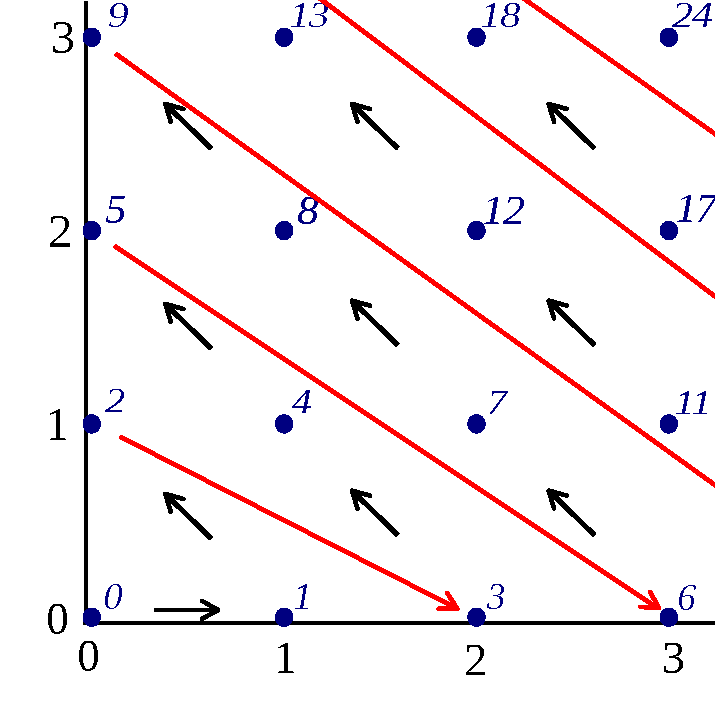
\includegraphics[width=0.6\textwidth]{files/diagcouples.pdf}
\caption{La fonction de couplage de Cantor établit une bijection de $\mathbb{N}*\mathbb{N}$ dans
 $\mathbb{N}$.}
 \end{center}
\end{figure*}

Soit $(x,y) \in \mathbb{N}*\mathbb{N}$ un couple. On trie par ordre lexicographique $(x+y)$. Ainsi on obtient le tableau suivant :

\begin{tabularx}{1.1\textwidth}{| m{1.5cm} | X | X | X | X | X | X | X | X | X | X | X }
\hline
$(x,y)$ & $(0,0)$ & $(1,0)$ & $(0,1)$ & $(2,0)$ & $(1,1)$ & $(0,2)$ & $(3,0)$ & $(2,1)$ & $(1,2)$ & $(0,3)$ & \ldots \\
\hline
$(x+y)$ & 0 & 1 & 1 & 2 & 2 & 2 & 3 & 3 & 3 & 3 & \ldots \\
\hline
$c_2(x+y)$ & 0 & 1 & 2 & 3 & 4 & 5 & 6 & 7 & 8 & 9 & \ldots \\
\hline
\end{tabularx}

\item
\begin{description}
\item[Fonction de codage]
\[ c_2(x,y)= \frac{(x+y)(x+y+1)}{2}+y \]

\item[Fonctions de décodage]
Les fonctions de décodage ne peuvent pas être décrites sous la forme de formules arithmétiques. Elles nécessitent l'algorithme suivant :

\begin{algorithm}[H]
  \caption{CalculXY($z$)}
  \Donnees{
  $z$ \textit{// Rang du couple (x,y)}
  }
  \Deb{
  $s \leftarrow 0$\;
  $t \leftarrow 0$\;
    \Tq{$s \leqslant z$}{
		$s \leftarrow \frac{t*(t+1)}{2}$\;
		$t \leftarrow t+1$\;
    }
    $t \leftarrow t-2$\;
    $z \leftarrow \frac{t*(t+1)}{2}$\;
    $y \leftarrow z-s$\;
    $x \leftarrow t-y$\;
    \Retour Couple($x$,$y$)\;
  }
\end{algorithm}
\end{description}

\item 
\begin{description}
\item[Codage des triplets] : il peut avoir lieu de manière récursive :
\[ c_3(x,y,z)=c_2(x,c_2(y,z)) \]
\item[Généralisation au codage des k-uplets] : 
\begin{eqnarray*}
& &c_k(x_1,x_2,\ldots,x_k)=c_2(x_1,c_{k-1}(x_2,\ldots,x_k)) \\
\textrm{Avec : } & &c_2(x,y)=\frac{(x+y)(x+y+1)}{2}+y
\end{eqnarray*}



\end{description}

\item Prenons une suite $r=(r_1,r_2,r_3,\ldots)$ qui énumère les réels de l'intervalle $[0;1]$, puis créons un réel x compris dans cet intervalle, tel que si la n\up{ième} de $r_n$ est égale à $1$, la n\up{ième} décimale de $x$ est égale à 2. Dans la cas contraire, la n\up{ième} décimale de $x$ est égale à 1.

On obtient sur cet exemple :

\begin{tabular}{r c c c c c c c c c c c c}
$r_1$ & = &0&,&\textbf{4}&2&9&6&4&6&1 &\ldots\\
$r_2$ & = &0&,&2&\textbf{7}&3&2&9&4&0 &\ldots\\
$r_3$ & = &0&,&6&4&\textbf{1}&1&5&1&2 &\ldots\\
$r_4$ & = &0&,&3&0&5&\textbf{9}&0&4&3 &\ldots\\
$r_5$ & = &0&,&9&1&3&3&\textbf{1}&8&2 &\ldots\\
$r_6$ & = &0&,&0&2&0&8&3&\textbf{2}&7 &\ldots\\
$r_7$ & = &0&,&2&5&7&3&6&4&\textbf{0} &\ldots\\
\vdots & \vdots & \vdots & \vdots & \vdots & \vdots & \vdots & \vdots & \vdots & \vdots & \vdots & $\ddots$ \\
&&&&$\downarrow$ &$\downarrow$ &$\downarrow$ &$\downarrow$ &$\downarrow$ &$\downarrow$ &$\downarrow$ &\\
$x$ & = &0&,&1&1&2&1&2&1&1&\ldots\\
\end{tabular}

Le réel $x$ ne peut pas être énuméré par la suite $r$ car il diffère de sa première décimale dans $r_1$, de sa deuxième décimale dans $r_2$, \ldots de sa n\up{ième} décimale dans $r_n$. Pourtant le réel $x$ est clairement dans l'intervalle $[0;1]$.

L'ensemble des éléments de l'intervalle $[0;1]$ ne sont donc pas dénombrables, donc pas énumérables. On ne peut donc pas trouver de fonction de codage pour cet ensemble.

On peu généraliser à l'ensemble $\mathbb{R}$ : $[0;1]$ étant inclus dans $\mathbb{R}$, et $[0;1]$ n'étant pas dénombrable, l'ensemble $\mathbb{R}$ n'est pas dénombrable.

\end{enumerate}
\clearemptydoublepage
\chapter{Partie pratique}
\textit{Le but de ce TP est d'implémenter deux algorithme de résolution du problème de flot maximum : l'algorithme d'Edmonds-Karp et l'algorithme de Dinic. Nous commencerons par spécifier les fonctionnalités que devra implémenter notre programme, puis nous détaillerons la manière dont ces fonctionnalités ont été développées. Une troisième partie sera consacrée aux tests effectués sur les deux algorithmes ainsi qu'à l'analyse des résultats.}

\section{Spécification fonctionnelles}

\subsection{Résolution du problème de flot maximum}

Le programme doit être capable de :
\begin{itemize}
\item générer et d'actualiser les graphes d'écarts successifs
\item calculer la valeur du flot obtenu à partir du graphe d'écart final
\item résoudre le problème de flot maximum en suivant l'algorithme d'\textbf{Edmonds-Karp}
\item résoudre le problème de flot maximum en suivant l'algorithme de \textbf{Dinic}
\item retourner la solution de manière exploitable pour l'analyse
\end{itemize}

Il faudra veiller à conserver les complexités des deux algorithmes, notamment en prenant garde aux structures de données et librairies utilisées.

\subsection{Génération aléatoire d'un réseau de transport}

La génération aléatoire de graphes de type réseau de transport permettra de tester les deux algorithmes. Il faudra veiller à ce que le graphe respecte les conditions d'un réseau de transport notamment la possession d'une source et d'un puits, la pondération des arcs (capacités), et assurer la connexité du graphe. La génération de ce réseau de transport devra être paramétrable selon la taille (nombre de sommets) et la couverture (nombre d'arcs).

\section{Spécification technique}

\subsection{Programmation C++}
Parce qu'il s'agit d'un bon compromis entre langage orienté objet et langage de bas niveau, nous avons choisi de développer cette application en C++. Nous pourrons ainsi abstraire la gestion des graphes (notamment des structures de données) dans nos algorithmes, tout en gardant la possibilité d'optimiser le code grâce à la flexibilité du langage C.

\subsection{Structures de données}

Plusieurs structures de données sont possibles. Nous avons choisi d'implémenter une représentation par listes d'adjacences et une autre par matrice d'adjacences.
\begin{description}
\item[Listes d'adjacences] : chaque sommet possède la liste de ses voisins. Ces listes ont l'avantage d'allouer de la mémoire uniquement lorsqu'une information doit être stockée. 
\item[Matrice d'adjacences] : la mémoire allouée pour cette structure de données ne dépend que du nombre de sommets ($n^2$). Cette structure a l'avantage d'offrir un accès direct à un arc pour deux sommets donnés.
\end{description}

Dans un but d'optimisation mémoire, on utilise en général des listes d'adjacences lorsque l'on travail sur des graphes peu denses. En effet, la taille allouée par cette structure de données étant directement dépendante du nombre d'arcs, elle est donc réduite par rapport aux matrices d'adjacences. Sur des graphes très dense, on utilisera plutôt des matrice d'adjacences, permettant un accès aux données plus rapide. 

Ce choix s'effectue en général en fonction des ressources matériels disponibles.

\subsection{Modélisation}
Dans un but d'abstraction de la structure de donnée, nous avons choisi de créer une classe abstraite \texttt{AbstractGraph} dont deux classes fille héritent. Un graphe peut donc être de type \texttt{AdjacencyListGraph} ou \texttt{MatrixGraph}. Cela permet une grande généricité des algorithme développés, ce qui permet d'utiliser une structure de données de manière totalement détachée des algorithmes.
\begin{figure}[t]
\begin{center}
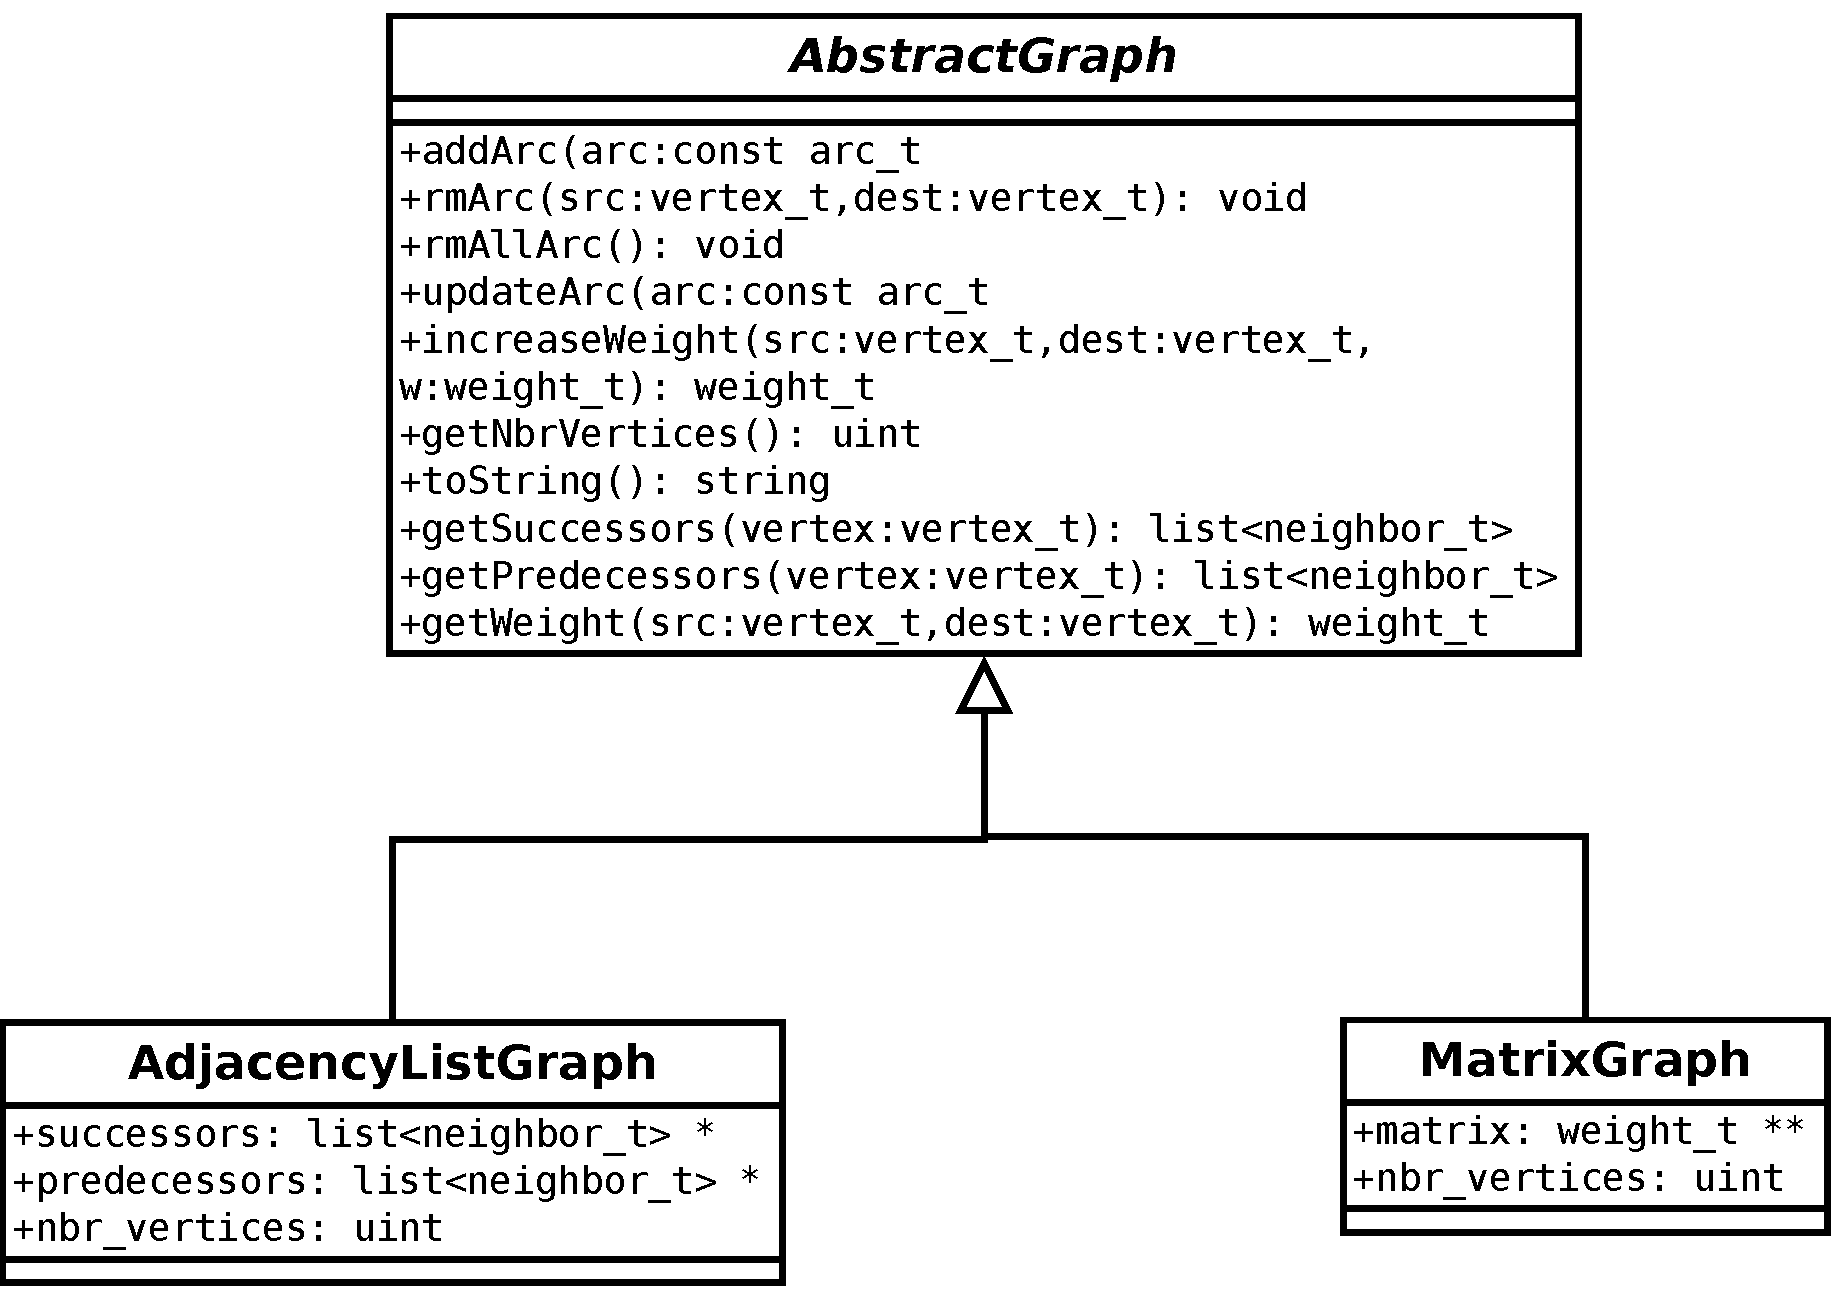
\includegraphics[width=\textwidth]{files/diag_class}
\end{center}
\caption{Diagramme de classes.}
\end{figure}

\FloatBarrier
\subsection{Implémentation}

\subsubsection{Types et structures}

Déclaration des types \texttt{weight\_t}, \texttt{vertex\_t} et \texttt{path\_t}, et des structures \texttt{edge}, \texttt{neighbor\_t}

\lstinputlisting[language=C++,morekeywords={}]{./sources/structs}

\subsubsection{Classe \texttt{AbstractGraph}}

Cette classe déclare une série de méthodes qui doivent êtres implémentés dans les classes filles.

Header de la classe \texttt{AbstractGraph}

\lstinputlisting[language=C++,morekeywords={}]{./sources/AbstractGraph}

\subsubsection{Classe \texttt{AdjacencyListGraph}}
Cette classe représente un réseau de transport sous la forme
de deux listes d'adjacences : une représente les 
successeurs d'un sommet, l'autre les prédécesseurs.

Ce doublon d'information permet d'accélérer l'accès aux voisins d'un sommet, notamment à ces prédécesseurs. En effet, cette méthode nous permet d'accéder aux prédécesseurs directement (complexité de $O(m)$) alors que l'accès via la liste des successeurs implique une recherche des arcs pour chaque sommet (complexité de $O(nm)$).

Ces doubles listes d'adjacences nous assurent un gain de performances en terme de rapidité, qui se fait au détriment de la quantité de mémoire utilisé, qui se trouve doublée.

Header de la classe \texttt{AdjacencyListGraph}

\lstinputlisting[language=C++,morekeywords={}]{./sources/AdjacencyListGraph}


\subsubsection{Classe \texttt{MatrixGraph}}

Header de la classe \texttt{MatrixGraph}

\lstinputlisting[language=C++,morekeywords={}]{./sources/MatrixGraph}

\section{Génération de réseaux de transport aléatoires}

\lstinputlisting[language=C++,morekeywords={}]{./sources/aleatoire}

\section{Procédures principales}

\subsection{Algorithme de Dinic}
\subsubsection{Mise à jour du graphe d'écart}
\lstinputlisting[language=C++,morekeywords={}]{./sources/ecart}

\subsubsection{Calcul du flot bloquant}
\lstinputlisting[language=C++,morekeywords={}]{./sources/bloquant}

\subsubsection{Exécution de Dinic}
\lstinputlisting[language=C++,morekeywords={}]{./sources/dinic}


\section{Tests \& résultats}

\subsection{Méthode de test}

\subsubsection{Série de tests}
Pour tester les performances des deux algorithmes implémentés, nous avons générer une série de problèmes à résoudre sur des réseaux de transports ayant les paramètres suivants :
\begin{itemize}
\item nombre de sommets variant de 100 à 1000 par palier de 100,
\item densité du graphe variant de 10\% à 100\% par palier de 10.
\end{itemize}
Pour chaque test (un nombre de sommets et une densité donnés), nous avons généré dix graphes afin de travailler sur des moyennes lors de l'analyse.

\subsubsection{GNU gprof}
Nous avons évalué les algorithmes en fonction de leurs temps d'exécution. Le temps réel d'exécution (real time) ayant peu de sens pour effectuer des statistiques correctes, nous avons choisi de mesurer les temps CPU (CPU time). Le temps CPU est le temps alloué au processus par le système d'exploitation sur le processeur. Contrairement au temps réel, le temps CPU est indépendant des autres processus en cours d'activité et aux interruptions systèmes : il s'agit du temps effectivement passé par le CPU pour traiter le processus.

L'analyse des temps CPU a été faite à l'aide de l'outil GNU gprof. Son utilisation requière l'ajout de l'argument \texttt{-pg} lors la compilation. A l'exécution du programme, un fichier \texttt{gmon.out} est généré. La commande \texttt{gprof} permet ensuite de créer un fichier texte de statistiques. Pour chaque méthode, un grand nombre de données sont disponibles, nous nous sommes intéressés principalement aux suivantes :
\begin{itemize}
\item pourcentage du temps CPU total,
\item temps CPU total,
\item temps CPU par appel, de manière cumulative (en prenant en compte les appel à d'autres fonctions) ou non.
\end{itemize}

\subsection{Analyse des résultats}



\end{document}